\section{Threat Model}
\begin{figure}
    \centering
    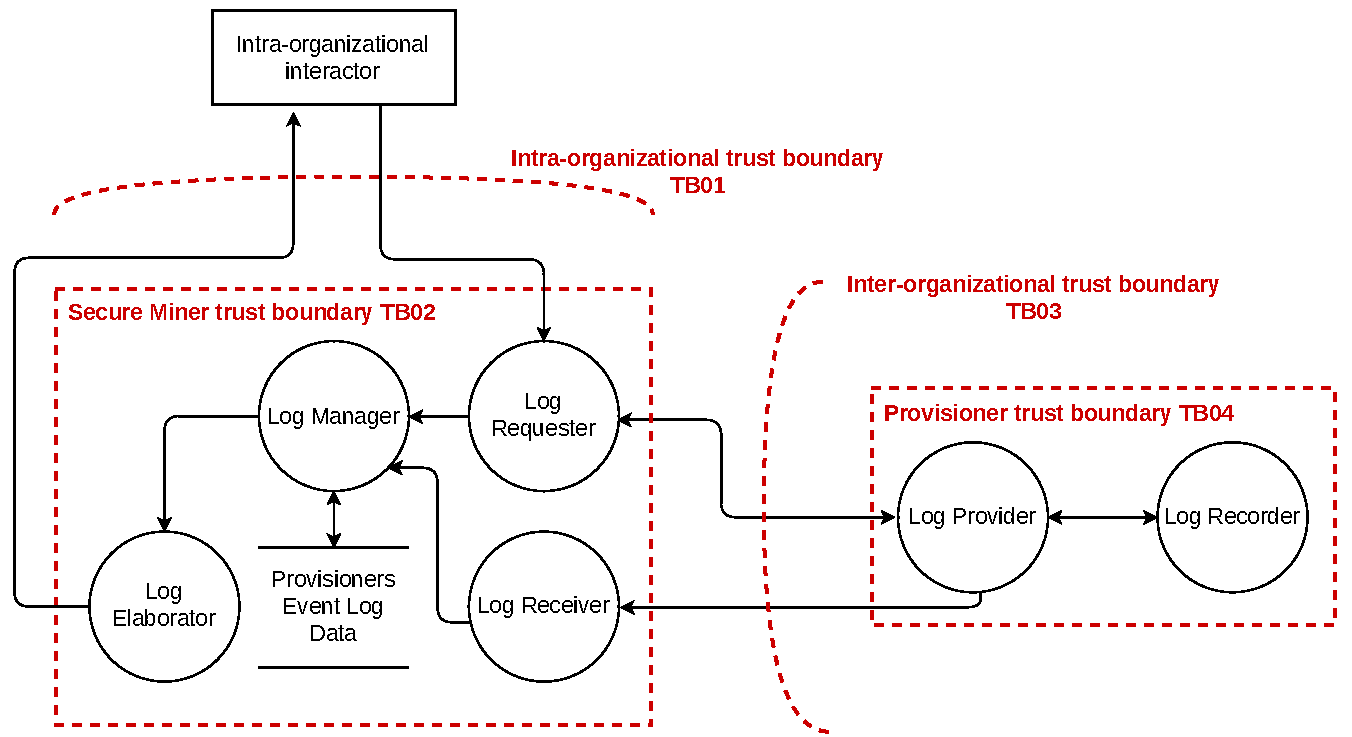
\includegraphics[width=0.95\linewidth]{content//figures/threatmodel.pdf}
    \caption{Data flow diagram employed for our threat model}
    \label{fig:threatmodel:dataflow}
\end{figure}
\begin{table}[t]
\label{table:threatmodel:threats}
\resizebox{\textwidth}{!}{%
    \centering
    \begin{tabular}{llll}\toprule
        \textbf{ID} & \textbf{Trust boundary}& \textbf{Type}  & \textbf{Threat description}\\ \midrule
        T01& \multirow{3}{*}{\makecell[l]{TB01}}& Spoofing   & The attacker impersonates a legitimate interactor to use the \Compo{Secure Miner}\\
        T02&     & Tampering  & The intra-organizational interactor sends malicious input to the \Compo{Secure Miner}\\
        T03&     & Information disclosure  & The attacker sniffs the messages between the interactor and the \Compo{Secure Miner}\\ \midrule
        T04& \multirow{4}{*}{\makecell[l]{TB02}}& Information disclosure  & The attacker accesses the \Compo{Secure Miner}'s memory location to leak the event logs\\ 
        T05& & Tampering  & The attacker meddles the source code of the \Compo{Secure Miner} or its event log data\\
        T06& & Elevation of privileges  & The attacker gains the rights to run in the same environment of the \Compo{Secure Miner}\\
        T07& & Denial of service  & The \Compo{Secure Miner} crashes, halts or stops\\ \midrule
        T08& \multirow{6}{*}{\makecell[l]{TB03}}& Spoofing  & The attacker impersonates a \Compo{Secure Miner} to gain access to the \Compo{Provisioner}'s log\\ 
        T09& & Spoofing  & The attacker impersonates a \Compo{Provisioner} to communicate with the \Compo{Secure Miner}\\
        T010& & Denial of service &The \Compo{Secure Miner} floods the \Compo{Provisioner} with log requests\\
        T010& & Denial of service &The \Compo{Secure Miner} floods the \Compo{Provisioner} with log requests\\
        T011& & Information disclosure & The attacker sniffs the \Compo{Provisioner}'s log sent to the \Compo{Secure Miner}\\ 
        T012& & Tampering & The attacker alters the data flow between the \Compo{Provisioner} and the \Compo{Secure Miner}\\
        \bottomrule
        
    \end{tabular}
    \caption{Vulnerabilities in the CONFINE architecture}
}
\end{table}
\begin{newj}
	

In the following section, we identify the threats that can jeopardize the proper functioning of CONFINE. Our threat analysis is based upon the theoretical foundation of the \textit{STRIDE} framework \cite{aa}. This conceptual model groups the threats into six categories: spoofing (i.e., the impersonation of a legitimate entity), tampering (i.e., the modification of data to alter its integrity), repudiation (i.e., the denial of performing a particular action), information disclosure (i.e., the exposure of sensitive data), denial of service (i.e., the disruption or degradation of availability) and elevation of privileges (i.e., the misappropriation of higher level of rights). 

With the help of the dataflow depicted in \cref{fig:threatmodel:dataflow}, we demarcate the \textit{trust boundaries} among the CONFINE components. In our diagram, a trust boundary box (a red dashed square) groups entities with mutual trust. Differently, trust boundary archs (a red dashed curved lines) mark the transitions of trust level on the occassion of data exchanges between mutually untrusted interactors. We identified the three main trust boundaries: intra-organizational trust boundary TB01, the Secure Miner's trust boundary (TB02), and the inter-organizational trust boundary (TB03). As a result of our analysis, we collect in \cref{table:threatmodel:threats} the CONFINE threats according to the STRIDE taxonomy.

As follow, we address the identified threats grouping them according to the threat boundary they refer to. 
	
%The trust boundary box TB02 groupes the components of the \Compo{Secure Miner}. The spectrum of the possible attacks to this boundary aims at breaking the isolation layer separating the \Compo{Secure Miner}'s component from untrusted entities. In order to disclosure the \Compo{Secure Miner}'s confidential information, a malicious actor may get access to the memory portion allocated to the \Compo{Secure Miner} (e.g., via Direct Memory Access attack) revealing event log's sensitive information (\textbf{T04}). Tampering threats manifest as the manipulation of the \Compo{Secure Miner}'s source code and event log data to generate misbehaviours or introducing vulnerabilities (\textbf{T05}). Furthermore, a malicious actor could acquire the necessary privileges (e.g., via kernel exploits) to execute code within the isolated context of the \Compo{Secure Miner}, potentially leading to unauthorized access or malicious code injection (\textbf{T06}). A denial-of-service attack may be employed a malicious entity to crash, halt, or disrupt the functioning of the \Compo{Secure Miner}, thereby impeding its ability to correctly aggregate event logs data and provide output analytics (\textbf{T07}).
The trust boundary box TB02 encompasses the components of the \Compo{Secure Miner}. The spectrum of potential attacks against this boundary is directed at compromising the isolation layer that separates the components of the \Compo{Secure Miner} from untrusted entities. To expose the confidential information within the \Compo{Secure Miner}, a malicious actor might gain access to the memory allocated to the \Compo{Secure Miner}, for instance, through a Direct Memory Access attack, thereby revealing sensitive information in the event logs (\textbf{T04}). Tampering threats materialize in the form of manipulating the \Compo{Secure Miner}'s source code and event log data to induce misbehaviors or introduce vulnerabilities (\textbf{T05}). Furthermore, a malicious actor could obtain the necessary privileges, such as through kernel exploits, to execute code within the isolated context of the \Compo{Secure Miner}, potentially resulting in unauthorized access or the injection of malicious code (\textbf{T06}). A denial-of-service attack may be employed by a malicious entity to crash, halt, or disrupt the functioning of the \Compo{Secure Miner}, thereby hindering the aggregation event log data correctly and the outsourcing of result analytics(\textbf{T07}). 

TB01 specifies the between the \Compo{Secure Miner} and any generic interactor in the same organization. 
\todo[inline]{
Introduce \cref{fig:threatmodel:dataflow} adoption;\\
Describe each boundary box with their adversary type (Provisioner --> honest, Secure Miner and input sources--> semi-honest)\\
Explain TB02 AND TB01;\\
For each TBi: describe all the STRICE threats that are in our scope
}

\end{newj}


